Le modèle standard de la cosmologie offre un formalisme décrivant l'évolution de l'Univers, du \textit{Big Bang} à aujourd'hui.
Ses succès observationnels sont nombreux, de l'expansion de l'Univers à l'existence du fond diffus cosmologique, en passant par la nucléosynthèse primordiale; aujourd'hui, il n'existe pas d'observations le mettant en échec.
Dans ce cadre, les propriétés de l'Univers sont décrites par un nombre restreint de quantités, nommées paramètres cosmologiques, dont la mesure est aujourd'hui l'enjeu de la cosmologie observationnelle.
Cette thèse s'inscrit dans ce cadre, et propose en particulier de contribuer à l'étude des mesures des paramètres cosmologiques en utilisant les amas de galaxies comme sondes cosmologiques.

Ce chapitre décrit les éléments nécessaires à la compréhension des analyses cosmologiques basées sur des amas de galaxies.
Nous commençons par présenter le modèle $\Lambda {\rm CDM}$, ou modèle standard de la cosmologie, décrivant le lien entre le contenu de l'Univers et sa dynamique.
Nous décrivons ensuite la formation des grandes structures, de leur origine à l'issue de l'inflation à leur développement récent par croissance des instabilités.

% ===================================================================================== %
\section{Le modèle standard de la cosmologie}

% ------------------------------------------------------------------------------------- %
\subsection{Les équations de Friedmann}\label{sec:friedmann}

La cosmologie moderne décrit l'Univers comme un objet dynamique obéissant aux lois de la relativité générale.
Ce cadre permet de lier la structure de l'espace-temps avec le contenu de l'Univers au travers des équations d'\myciteauthor{einstein_feldgleichungen_1915}:
\begin{equation}
    \label{eq:einst_field}
    G_{\mu\nu} - \Lambda g_{\mu\nu} = \frac{8\pi G}{c^4} T_{\mu\nu}.
\end{equation}
La partie gauche de l'équation encode la géométrie de l'espace-temps au travers du tenseur d'Einstein $G_{\mu\nu}$ et de la métrique $g_{\mu\nu}$, et la partie droite décrit la dynamique des composants de l'Univers par leur tenseur énergie-impulsion $T_{\mu\nu}$.
$G$ est la constante gravitationnelle Newtonienne, $c$ la vitesse de la lumière dans le vide, et $\Lambda$ la constante cosmologique, qui sera discutée en section \ref{sec:dark_energy}.
Dans l'hypothèse d'un Univers globalement homogène et isotrope, la solution dynamique la plus simple de l'équation (\ref{eq:einst_field}) est donnée par la métrique de Friedmann–Lemaître–Robertson–Walker (FLRW):
\begin{equation}
    \label{eq:flrw}
    \d s^2 = g_{\mu\nu} \d x^\mu \d x^\nu = c^2 \d t^2 - a^2(t) \left[ \frac{1}{1 - kr^2} \d r^2 + r^2 \d\theta^2 + r^2 \sin^2\theta \, \d\phi^2 \right],
\end{equation}
où $(t, r, \theta, \phi)$ sont les coordonnées sphériques à quatre dimensions. \\
Le paramètre de courbure $k$ caractérise la géométrie globale de l'Univers, qui peut être hyperbolique ($k=-1$), sphérique ($k=1$), ou plate ($k=0$, cas favorisé par les observations).
La fonction $a(t)$ est le facteur d'échelle de l'Univers, décrivant son expansion.
Son expression peut être écrite en considérant le contenu de l'Univers comme un fluide parfait comobile de densité d'énergie $\rho$ et de pression $p$, dont le tenseur énergie-impulsion s'écrit en fonction de la quadri-vitesse du fluide $u^\mu$
\begin{equation}
    \label{eq:tmunu}
    T^{\mu\nu} = (p/c^2 + \rho)u^\mu u^\nu - p g^{\mu\nu}.
\end{equation}
Alors, la combinaison des équations (\ref{eq:einst_field}), (\ref{eq:flrw}) et (\ref{eq:tmunu}) permet d'aboutir aux équations de Friedmann:
\begin{equation}
    \label{eq:fried1}
    H^2(t) \equiv \left(\frac{\dot{a}}{a}\right)^2 = \frac{8\pi G}{3} \rho + \frac{\Lambda c^2}{3} - \frac{kc^2}{a^2}
\end{equation}
\begin{equation}
    \label{eq:fried2}
    \frac{\ddot{a}}{a} = -\frac{4\pi G}{3} \left(\rho + \frac{3}{c^2} p\right) + \frac{\Lambda c^2}{3}
\end{equation}
où $\dot{a}$ dénote la dérivée temporelle de $a$, et $H(t)$ est le paramètre de Hubble, quantifiant le taux d'expansion de l'Univers.

Ces équations différentielles lient la dynamique de l'Univers à l'évolution de la densité d'énergie et de pression de son contenu.
Cette évolution dépend du paramètre d'équation d'état $w=p/(\rho c^2)$ du fluide: la combinaison des équations (\ref{eq:fried1}) et (\ref{eq:fried2}) donne l'équation de conservation de l'énergie pour un fluide parfait comobile,
\begin{equation}
    \dot{\rho} = -3(\rho + p/c^2) \times H(t),
\end{equation}
et donc l'évolution avec le facteur d'échelle de la densité d'énergie $\rho$:
\begin{equation}
    \label{eq:rho_w}
    \rho(a) \propto a^{-3(1+w)}
\end{equation}
Le contenu de l'Univers peut être séparé en plusieurs fluides parfaits comobiles, notés $j$, représentant les différents constituants de l'Univers, et possédant chacun un paramètre d'état $w_j$.
Ces constituants sont la matière, comprenant l'ensemble des baryons de l'Univers, ainsi que la matière sombre, et le rayonnement, composé des photons et autres espèces relativistes de l'Univers.
L'équation de Friedmann (\ref{eq:fried1}) peut s'écrire en fonction des densités $\rho_j$ des différents constituants $j$ de l'Univers:
\begin{equation}
    H^2(a) = \frac{8\pi G}{3 }\sum_j \rho_j(a) + \frac{\Lambda c^2}{3} - \frac{kc^2}{a^2}.
\end{equation}
Ainsi, en introduisant la densité critique $\rho_c$ comme:
\begin{equation}
    \label{eq:rho_crit}
    \rho_c(a) \equiv \frac{3 H^2(a)}{8 \pi G},
\end{equation}
on peut définir les abondances relatives de chaque composante comme $\Omega_j \equiv \rho_j / \rho_c$.
La constante cosmologique et la courbure peuvent donc être considérées comme des constituants supplémentaires de l'Univers, d'abondances relatives respectives $\Omega_\Lambda \equiv \Lambda c^2 / 3H^2$ et $\Omega_k \equiv -kc^2 / (aH)^2$.
La première équation de Friedmann (\ref{eq:fried1}) s'écrit finalement:
\begin{equation}
    \label{eq:fried_omega}
    H^2(a) = H_0^2 \sum_i \Omega_{i,0} \, a^{-3(1+w_i)},
\end{equation}
où $H_0$ est le taux d'expansion actuel de l'Univers, et où les composantes $i$ comprennent les constituants précédemment notés $j$ (matière et rayonnement), ainsi que la courbure et la constante cosmologique.
Leurs abondances relatives actuelles sont notées $\Omega_{i,0}$.
Les différents constituants de l'Univers, leurs paramètres d'équation d'état, et leur abondances actuelles mesurées par l'analyse des anisotropies du fond diffus cosmologique (ou CMB pour \textit{Cosmic Microwave Background}) par le satellite \textit{Planck} \cite{planck_collaboration_planck_2020} sont résumés dans la table \ref{tab:cosmo_params}.

\begin{table}[t]
    \small
    \centering
    \begin{tabular}{c c c}
        \toprule
        Composante $i$ & $w_i$ & $\Omega_{i,0}$ \\
        \midrule
        Matière $m$                         & $0$     & $0.3111 \pm 0.0056$ \\
        Rayonnement $r$                     & $1/3$   & $\sim 10^{-5}$ \\
        Constante cosmologique $\Lambda$    & $-1$    & $0.6889 \pm 0.0056$ \\
        Courbure $k$                        & $-1/3$  & $0.0007 \pm 0.0019$ \\
        \bottomrule
    \end{tabular}
    \caption{%
        Paramètres d'état $w$ et abondances actuelles $\Omega_0$ des constituants de l'Univers issues de l'analyse des anisotropies du fond diffus cosmologique mesurées par \textit{Planck} \cite{planck_collaboration_planck_2020}.
    }
    \label{tab:cosmo_params}
\end{table}

% ------------------------------------------------------------------------------------- %
\subsection{Expansion de l'Univers, accélération et énergie sombre}
\label{sec:dark_energy}

Les équations de Friedmann permettent de lier l'évolution du facteur d'échelle de l'Univers aux densités d'énergie de ses différents constituants, et d'étudier cette évolution dans le temps.
D'après la combinaison de la première équation de Friedmann (\ref{eq:fried_omega}) et de l'équation (\ref{eq:rho_w}), il apparait que le facteur d'échelle d'un Univers de densité d'énergie dominée par un constituant $i$ d'équation d'état $w_i \geqslant -1$ ne peut qu'augmenter avec le temps\footnote{Dans la mesure où $\Omega_{i, 0}$ est positif.}.
Chacun des constituants de notre Univers vérifiant cette condition (comme montré en table \ref{tab:cosmo_params}), nous pouvons en déduire que celui-ci est en expansion.
Cette expansion se caractérise par une dilatation de l'espace-temps avec le temps, et une augmentation des distances séparant les différents objets présents dans l'Univers.
Il en découle que par le passé, l'Univers entier était contenu dans un volume bien plus faible qu'aujourd'hui, diminuant en remontant le temps jusqu'à atteindre une singularité de l'espace-temps: c'est le modèle du \textit{Big Bang}, élément majeur de notre compréhension de la cosmologie.

Historiquement, la constante cosmologique $\Lambda$ fût introduite par Einstein dans les équations du champ (\ref{eq:einst_field}) afin de pouvoir décrire un modèle d'Univers statique.
Cette hypothèse fût mise en échec par les confirmations observationnelles de l'expansion par \myciteauthor{lemaitre_univers_1927} et \myciteauthor{hubble_relation_1929}.
Ces études ont mis en évidence le décalage vers le rouge des spectres de galaxies l'expansion: un photon émis a un instant $t_1$ et à une longueur d'onde $\lambda_1$, verra sa longueur d'onde augmenter au cours de son voyage dans l'Univers de par la dilatation de l'espace-temps.
Ainsi, à un instant postérieur $t_0$, sa longueur d'onde $\lambda_0$ sera décalée vers les grandes longueurs d'onde -- et donc vers le rouge, décalage quantifié par le \textit{redshift} $z$:
\begin{equation}
    \label{eq:redshift}
    1 + z = \frac{\lambda_0}{\lambda_1} = \frac{a(t_0)}{a(t_1)}.
\end{equation}
Einstein retira alors son hypothèse d'Univers statique et la constante cosmologique, menant aux travaux sur le modèle cosmologique Einstein-de Sitter \cite{einstein_relation_1932} décrivant un univers en expansion continue avec $\Lambda = 0$.

Les modèles d'univers à constante cosmologique non-nulle ne refirent leur apparition que soixante ans plus tard, lorsque les observations de supernovas de type Ia par \myciteauthor{riess_observational_1998} et \myciteauthor{perlmutter_measurements_1999} mirent en évidence l'accélération récente de l'expansion de l'Univers.
En vertu de la deuxième équation de Friedmann (\ref{eq:fried2}), une telle accélération, caractérisée par $\ddot{a} > 0$, ne peut avoir lieu sans la présence d'un constituant de l'Univers de paramètre d'équation d'état $w < -1/3$.
Une nouvelle espèce fût donc ajoutée au contenu de l'Univers, génériquement nommée énergie sombre (\textit{dark energy}), d'abondance relative $\Omega_\textsc{de}$ et d'équation d'état $w_\textsc{de}$.
Dans le cas où $w_\textsc{de} = -1$, l'énergie sombre se comporte comme la constante cosmologique d'Einstein.
Les analyses cosmologiques actuelles, basées sur l'exploitation de différentes sondes pour mesurer les différents paramètres cosmologiques, sont toutes en accord avec la valeur de $w_\textsc{de} = -1$, faisant de la constante cosmologique un candidat à l'explication de l'origine de l'accélération de l'expansion.
Des modèles plus élaborés permettent au paramètre d'état de varier dans le temps, par exemple dans la paramétrisation CPL \cite{chevallier_accelerating_2001,linder_exploring_2003},
\begin{equation}
    \label{eq:de_cpl}
    w(a) = w_0 + (1-a) w_a,
\end{equation}
mais les incertitudes sur les mesures ne permettent actuellement pas de différencier de tels modèles d'une constante cosmologique.
De même, des modèles de gravitation modifiée cherchent à expliquer l'accélération en modifiant la relativité générale aux échelles cosmologiques, mais ne sont pour l'instant pas contraignables observationnellement (voir \cite{clifton_modified_2012,tamosiunas_testing_2020} pour des revues).

Le modèle actuellement adopté comme modèle standard de la cosmologie est le modèle $\Lambda{\rm CDM}$ pour \textit{Lambda Cold Dark Matter}, dans lequel l'énergie sombre est une constante cosmologique ($w_\textsc{de} = -1$), la matière sombre est non-relativiste, et l'Univers est plat ($\Omega_k = 0$).
Ses extensions les plus couramment considérées en cosmologie observationnelles sont:
\begin{itemize}[leftmargin=*]
    \setlength\itemsep{5pt}
\item le modèle $w{\rm CDM}$, dans lequel la densité d'énergie sombre peut varier dans le temps ($w_\textsc{de} \neq -1$);
\item le modèle $w_0 w_a {\rm CDM}$, extension du modèle $w{\rm CDM}$ dans laquelle le paramètre d'état de l'énergie sombre peut également varier dans le temps (voir équation \ref{eq:de_cpl});
\item le modèle $k{\rm \Lambda CDM}$, dans lequel l'Univers n'est pas nécessairement plat;
\item le modèle $\nu{\rm \Lambda CDM}$, dans lequel on considère la masse des neutrinos comme un paramètre cosmologique, du fait de l'importance de ceux-ci dans la formation des structures (voir par exemple \cite{lesgourgues_massive_2006} pour une revue).
\end{itemize}

% ------------------------------------------------------------------------------------- %
\subsection{Histoire thermique de l'Univers}

Le modèle standard de la cosmologie fournit une description du contenu de l'Univers et de son évolution dans le temps.
Quelques instants après le Big Bang, l'intégralité des constituants de l'Univers est contenue dans un volume très faible.
Il est alors rempli d'un gaz chaud ionisé de pression et température extrêmes, nommé plasma primordial, dans lequel les particules élémentaires sont toutes libres et en interaction constante.
La densité d'énergie est alors dominée par le rayonnement, et le facteur d'échelle évolue comme $a \propto t^{1/2}$.

Avec l'expansion, le volume de l'Univers augmente, permettant au plasma primordial de se diluer.
Sa densité, sa température et sa pression décroissent, diminuant ainsi les taux d'interaction des particules.
Les espèces interagissant le plus faiblement, comme les neutrinos et la matière sombre, commencent alors à se découpler du plasma primordial alors que leur taux d'interaction devient plus faible que le taux d'expansion de l'Univers.
Lorsque la température atteint $\sim 100 \;{\rm keV}$, les premiers noyaux se forment par interaction entre protons et neutrons: des noyaux de deutérium, hélium, puis lithium sont alors formés, marquant la nucléosynthèse primordiale (pour une revue du processus et de résultats récents, voir \cite{cyburt_big_2016}).

Alors que l'expansion continue son cours, la densité d'énergie du rayonnement décroit en $\rho_r \propto a^{-4}$, plus vite que celle de la matière qui diminue en $\rho_m \propto a^{-3}$ (cf. section \ref{sec:friedmann}).
L'Univers arrive donc dans une phase où la densité d'énergie de la matière domine, à partir d'un redshift de $z \sim 3400 \;(T \sim 10^4 \;{\rm K})$, soit quelques soixante mille ans après le Big Bang, et l'expansion continue avec $a \propto t^{2/3}$.
Par la suite, alors que le taux d'interactions continue de chuter, les premiers atomes d'hydrogène se forment par combinaison d'électrons avec les noyaux formés lors de la nucléosynthèse primordiale, constituant la recombinaison.
L'Univers devient alors neutre, et les photons peuvent se propager librement et se découplent: c'est l'émission du fond diffus cosmologique (ou CMB), à $z \sim 1000$.
Ce rayonnement constitue la première lumière émise dans l'Univers jusqu'alors opaque, et il constitue l'une des sondes majeures de la cosmologie.
Il se manifeste observationnellement comme un rayonnement dont le spectre est celui d'un corps noir de température $T_{\rm CMB} = 2.725 \; {\rm K}$ \cite{fixsen_cosmic_1996}, remarquablement homogène sur tout le ciel, présentant des fluctuations en température de l'ordre de $10^{-4} \;{\rm K}$.
Le spectre de puissance de ces fluctuations est intimement lié aux propriétés de l'Univers au moment du découplage des photons, et donc aux paramètres cosmologiques.

La matière s'arrange alors par effondrement gravitationnel autour des régions les plus denses, donnant naissance à la structure à grande échelle de l'Univers.
L'origine de ces fluctuations, de même que le processus de formation des structures, sera détaillée dans la section \ref{sec:struct_form}.
Enfin, à un redshift $z \sim 0.5$, la densité d'énergie de la matière devient plus faible que celle de l'énergie sombre, qui commence à dominer le contenu énergétique de l'Univers.
C'est alors que l'accélération de l'expansion commence.

Les grandes étapes de l'histoire thermique de l'Univers sont résumées sur la figure \ref{fig:cosmo:thermal_history}.
Celle-ci montre une représentation schématique de l'Univers au fur et à mesure de ces grandes étapes.
L'évolution du facteur d'échelle est représentée par l'agrandissement avec le temps (de gauche à droite) de la représentation de l'Univers.
Entre l'inflation et la recombinaison, l'Univers est opaque aux photons et très homogène.
Par la suite, la matière le composant se structure pour former la toile cosmique, composée de filaments séparés par des vides, et dont les intersections forment des pics de surdensité qui donneront naissance aux amas de galaxies: c'est la formation des grandes structures, qui sera détaillée dans la section suivante.
Les régions denses continuent par la suite à accréter de la matière, et deviennent de plus en plus denses, donnant lieu à la structure de l'Univers contemporain.

\vfill % bidouille

\begin{figure*}[t]
    \centering
    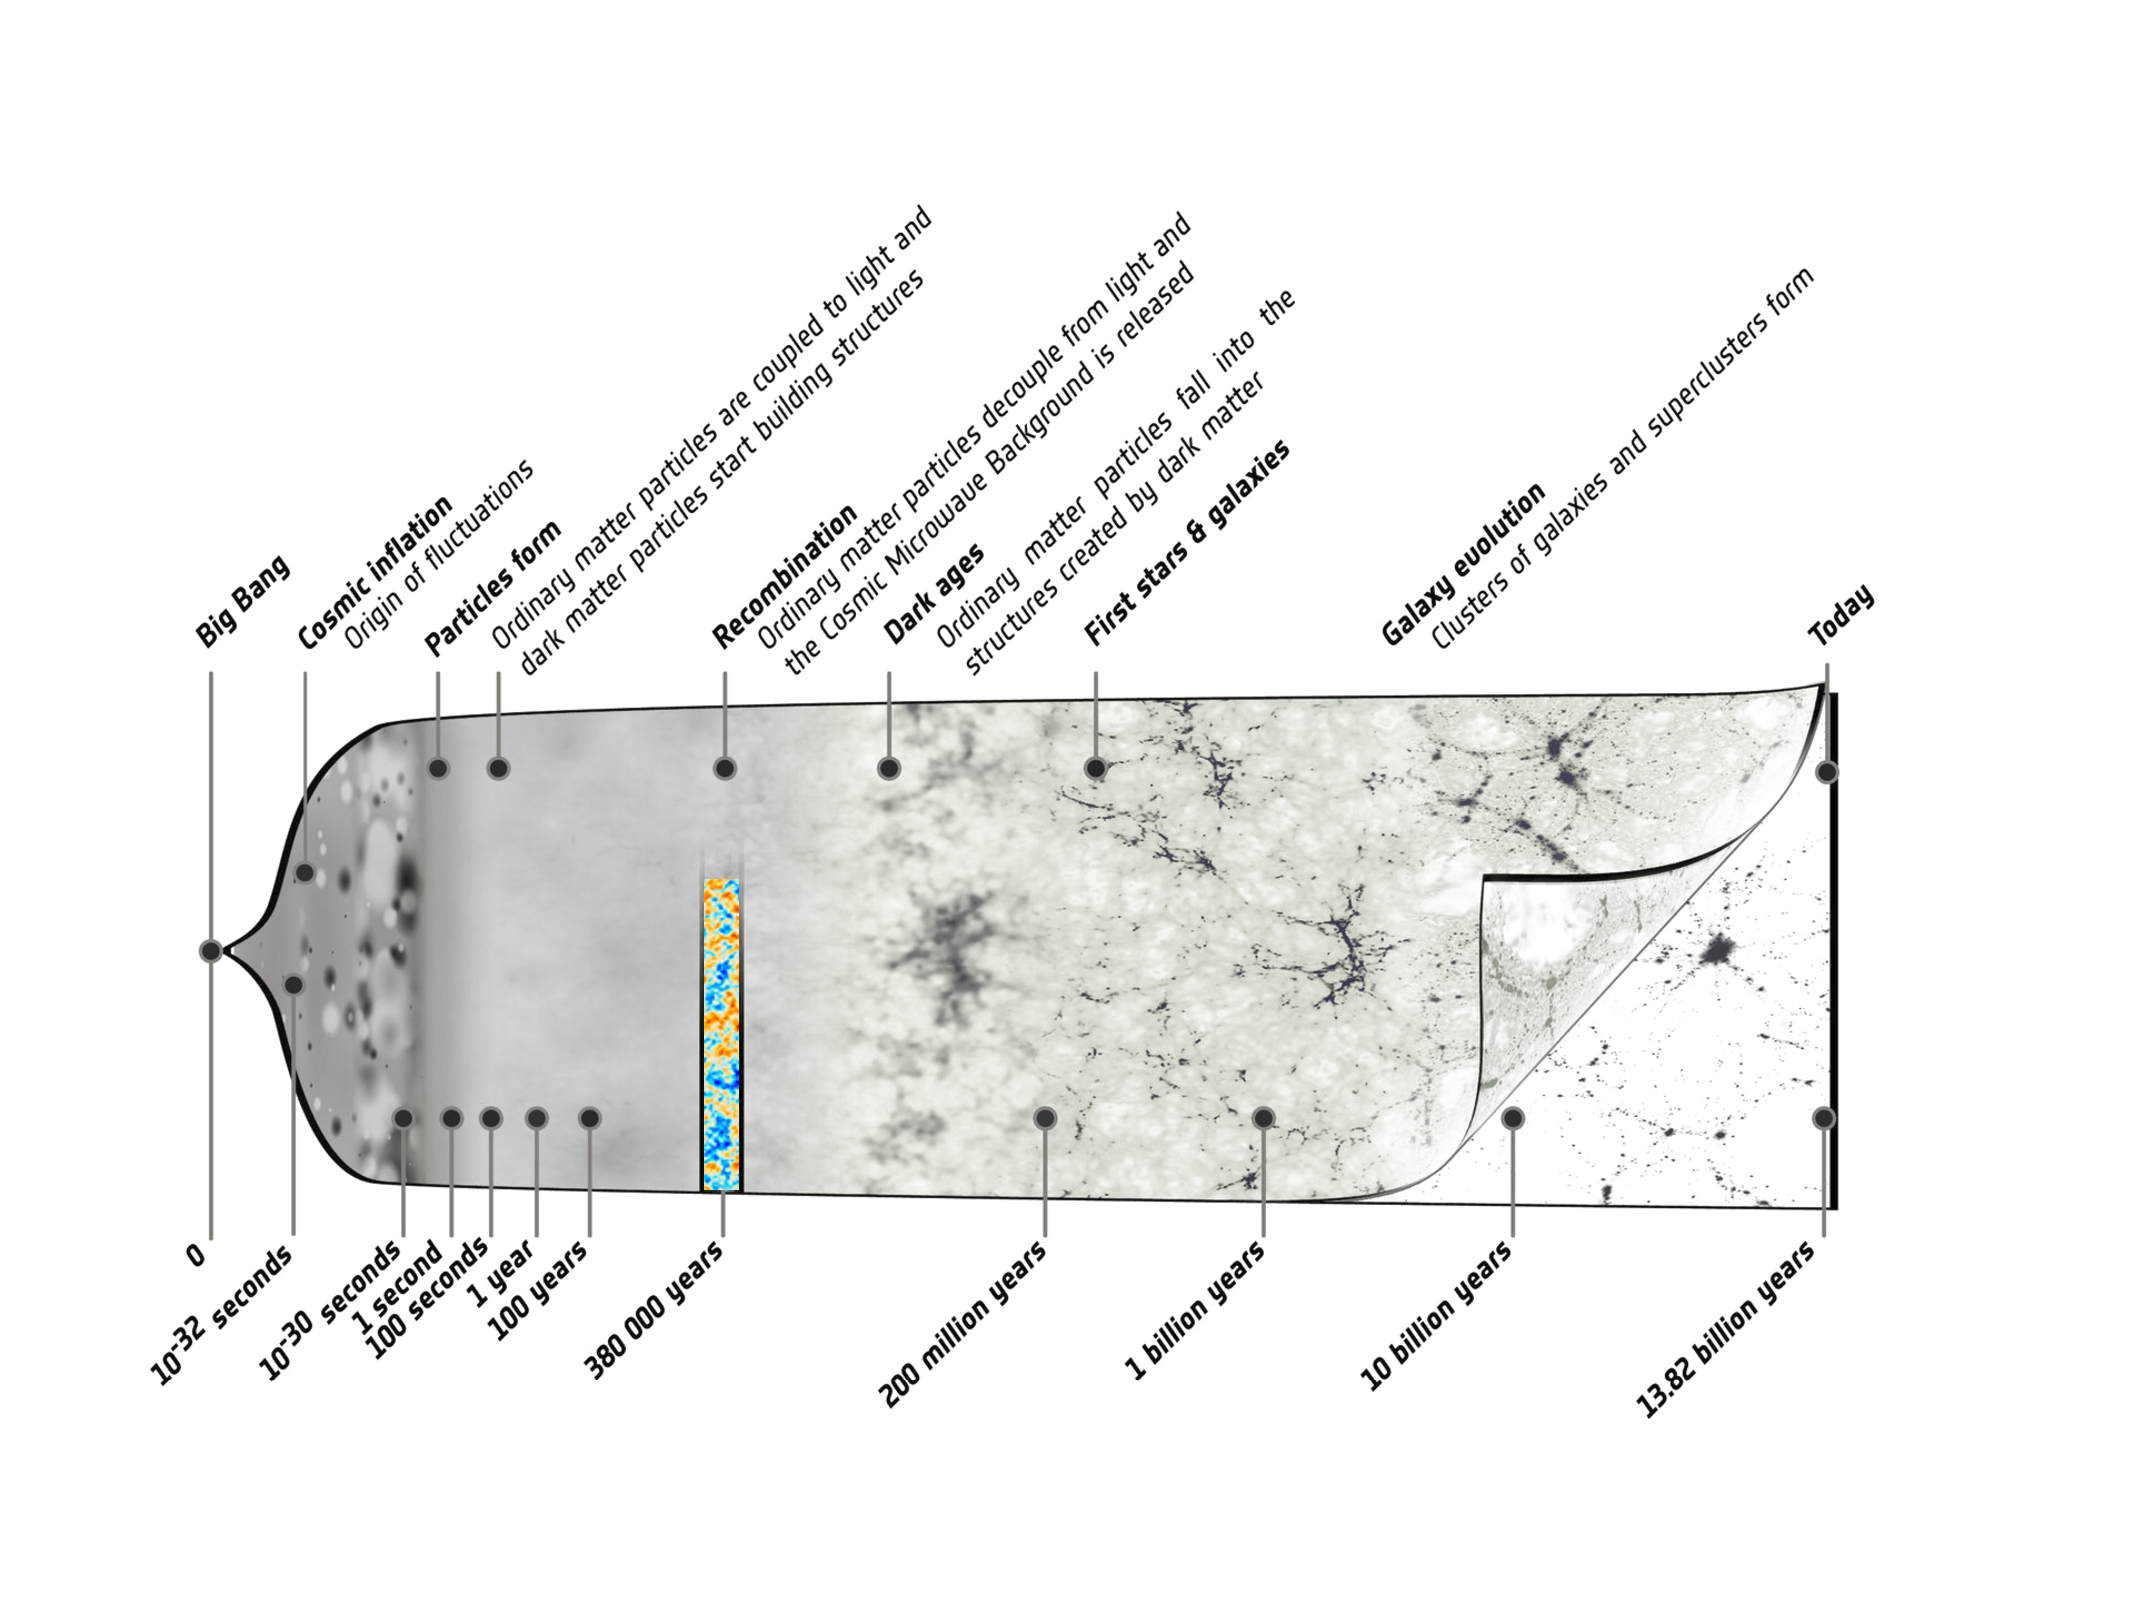
\includegraphics[width=.9\linewidth, trim={2cm 3cm 2cm 3cm}, clip]{Figures/Chap_cosmo/history_of_Universe.pdf}
    \caption{
        Résumé des étapes de l'histoire thermique de l'Univers, du Big Bang à aujourd'hui.
        Crédit: \href{https://www.esa.int/ESA_Multimedia/Images/2013/03/Planck_history_of_Universe_zoom}{ESA – C. Carreau}
    }
    \label{fig:cosmo:thermal_history}
\end{figure*}

% ===================================================================================== %
\section{Origine des grandes structures}\label{sec:struct_form}

Les équations de Friedmann permettent l'étude de la dynamique d'un univers homogène et isotrope.
La faible amplitude des fluctuations en température du CMB nous confirme l'isotropie à grande échelle de l'Univers.
Cependant, l'Univers contemporain est hautement hétérogène aux petites échelles, comme en témoigne l'existence de structures telles que les galaxies, amas de galaxies, étoiles et autres astres.
Notre Univers est donc homogène aux grandes échelles et hétérogène aux petites, ce qui n'est pas expliqué par le modèle standard de la cosmologie.
Nous décrivons dans cette section le paradigme inflationnaire, permettant de pallier aux lacunes du modèle standard, et offrant un cadre théorique pouvant expliquer l'origine de la formation des grandes structures de l'Univers.

% ------------------------------------------------------------------------------------- %
\subsection{Limitations du modèle standard de la cosmologie}

Bien que capable d'expliquer une grande variété de phénomènes observés dans l'Univers, le modèle $\Lambda\mathrm{CDM}$ est limité et ne fournit pas de réponse à certaines questions fondamentales de la cosmologie, parmi lesquelles:

\subsubsection{Le problème de l'homogénéité à grande échelle} % ----------------------- %
Les observations des anisotropies en température du fond diffus cosmologique nous indiquent que l'Univers était extraordinairement homogène au moment de son découplage 380 000 ans après le Big Bang, avec des fluctuations quatre ordres de grandeurs plus faibles que sa température moyenne.
Cette homogénéité peut s'expliquer par un équilibre thermique dans le plasma primordial.
Cependant, un tel équilibre requiert un contact causal entre les différentes régions de l'Univers, contact n'ayant pu exister au moment de l'émission du CMB au vu de la valeur du facteur d'échelle à cette époque.
Quantitativement, alors que le CMB est homogène sur tout le ciel (et donc pour des points séparés par des angles allant jusqu'à 180\textdegree), l'angle tendu par le rayon d'horizon de Hubble à cette époque est de l'ordre du degré.
Le modèle standard de la cosmologie ne permet donc pas d'expliquer l'homogénéité en température du fond diffus cosmologique.

\subsubsection{Le problème de l'hétérogénéité à petite échelle} % --------------------- %
Bien que remarquablement homogène à grande échelle, l'Univers est très hétérogène à petite échelle.
Le modèle cosmologique standard ne permet d'expliquer que partiellement ce constat: de faibles inhomogénéités dans l'Univers primordial peuvent croître avec l'expansion jusqu'à devenir les structures que nous connaissons.
Cependant, l'origine des fluctuations de densité primordiales nécessaires à ce développement n'est pas expliquée par le modèle cosmologique standard.

\subsubsection{Le problème de la platitude} % ----------------------------------------- %
Les analyses cosmologiques récentes, basées sur l'exploitation de différentes sondes, s'accordent à dire que la géométrie de l'Univers est extrêmement plate, correspondant à une densité d'énergie dans l'Univers très proche de la densité critique (équation \ref{eq:rho_crit}).
Une courbure aussi faible que celle mesurée par l'analyse des anisotropies du CMB avec \textit{Planck} ($\Omega_{k,0} \sim 10^{-3}$) nécessite une courbure inférieure à $10^{-60}$ à l'issue de l'ère de Planck\footnote{Premières $10^{-43}$ secondes de l'Univers.}.
Des contraintes aussi fortes requièrent donc un ajustement fin des propriétés physiques de l'Univers primordial pour qu'il puisse se développer en l'Univers contemporain que nous observons, sans que le modèle cosmologique standard n'offre d'explication.

% ------------------------------------------------------------------------------------- %
\subsection{Fluctuations primordiales et inflation}

Les problèmes d'homogénéité à grande échelle et de platitude peuvent être résolus par un même mécanisme: l'inflation.
Dans ce scénario, l'Univers primordial a subi une phase d'expansion accélérée très rapide, caractérisée par $\ddot{a} > 0$, soit:
\begin{equation}
    \frac{\d}{\d t} \frac{1}{aH} < 0
\end{equation}
La présence de faibles hétérogénéités dans l'Univers primordial, à l'origine du processus de formation des structures, peut également être expliquée dans ce cadre.

Le paradigme de l'inflation comprend un grand nombre de modèles visant à expliquer l'origine de l'expansion accélérée dans l'Univers primordial.
Dans sa forme la plus simple, l'inflation est due à un champ scalaire homogène $\varphi$ nommé \textit{inflaton}, faiblement couplé et de potentiel $V(\varphi)$, dont la densité d'énergie domine celles de la matière et du rayonnement dans l'Univers primordial, avant de s'effondrer.
Le Lagrangien de ce champ s'écrit
\begin{equation}
    \mathcal{L} = \frac{1}{2} \partial^\mu\varphi \, \partial_\mu\varphi - V(\varphi) = \frac{\dot{\varphi}^2}{2} - V(\varphi),
\end{equation}
et le tenseur énergie-impulsion de ce champ $T^{\mu\nu} = \partial^\mu\varphi \, \partial^\nu\varphi - \mathcal{L}g^{\mu\nu}$ prend alors la forme de celui d'un fluide parfait dont la densité et la pression s'écrivent
\begin{align}
    \label{eq:infla_dens_press}
    \nonumber \rho_\varphi c^2 &= \frac{\dot{\varphi}^2}{2} + V(\varphi)
    + \frac{1}{2}\left(\frac{\nabla\varphi}{a}\right)^2, \\
    p_\varphi &= \frac{\dot{\varphi}^2}{2} - V(\varphi)
    - \frac{1}{6}\left(\frac{\nabla\varphi}{a}\right)^2.
\end{align}
Dans une phase d'expansion rapide de l'Univers (comme au cours du \textit{slow-roll} discuté dans le paragraphe suivant), les termes proportionnels au gradient du champ d'inflaton $\nabla\varphi$ deviennent rapidement négligeables, du fait de la présence au dénominateur du facteur d'échelle.
La conservation du tenseur énergie-impulsion donne alors l'équation du mouvement de ce champ:
\begin{equation}
    \label{eq:infla_mvt}
    \ddot{\varphi} + 3H\dot{\varphi} + \frac{\d V(\varphi)}{\d\varphi} = 0.
\end{equation}

On peut alors distinguer deux régimes.
Dans le cas où $\ddot{\varphi}$ est négligeable devant les autres termes, l'énergie potentielle du champ d'inflaton domine son énergie cinétique: on dit que le champ se trouve dans une phase de \textit{slow-roll}\footnote{L'équation du mouvement (\ref{eq:infla_mvt}) est similaire à celle d'une balle dévalant une colline avec une friction non-nulle. Le \textit{slow-roll} correspond au roulement initial, où la friction domine et ralentit le mouvement -- voir figure \ref{fig:inflation}, panneau gauche.}.
On peut alors écrire $\dot{\varphi}^2 \ll V(\varphi)$, et le rapport de la densité d'énergie et de la pression du champ d'inflaton (équation \ref{eq:infla_dens_press}) donne un paramètre d'équation d'état $w_\varphi = -1$, caractéristique d'une expansion accélérée de l'Univers.
À l'inverse, si le terme cinétique domine par rapport au potentiel, l'équation du mouvement est celle d'un oscillateur harmonique amorti, et le champ se trouve dans une phase de \textit{reheating}.
Dans cette phase, l'oscillation du champ d'inflaton permet de convertir son énergie par production de particules élémentaires (\eg\ \cite{abbott_particle_1982,albrecht_reheating_1982}).

Le comportement de l'inflaton est illustré en figure \ref{fig:inflation}.
S'il se trouve dans une région de potentiel élevé, il se dirigera vers un potentiel plus faible en \textit{slow-roll}, générant l'inflation dans la région grisée.
Une fois proche d'un minimum de potentiel, le champ se trouvera dans une phase d'oscillations périodiques amorties avant de se stabiliser, mettant un terme à l'inflation.

\begin{figure*}[t]
    \centering
    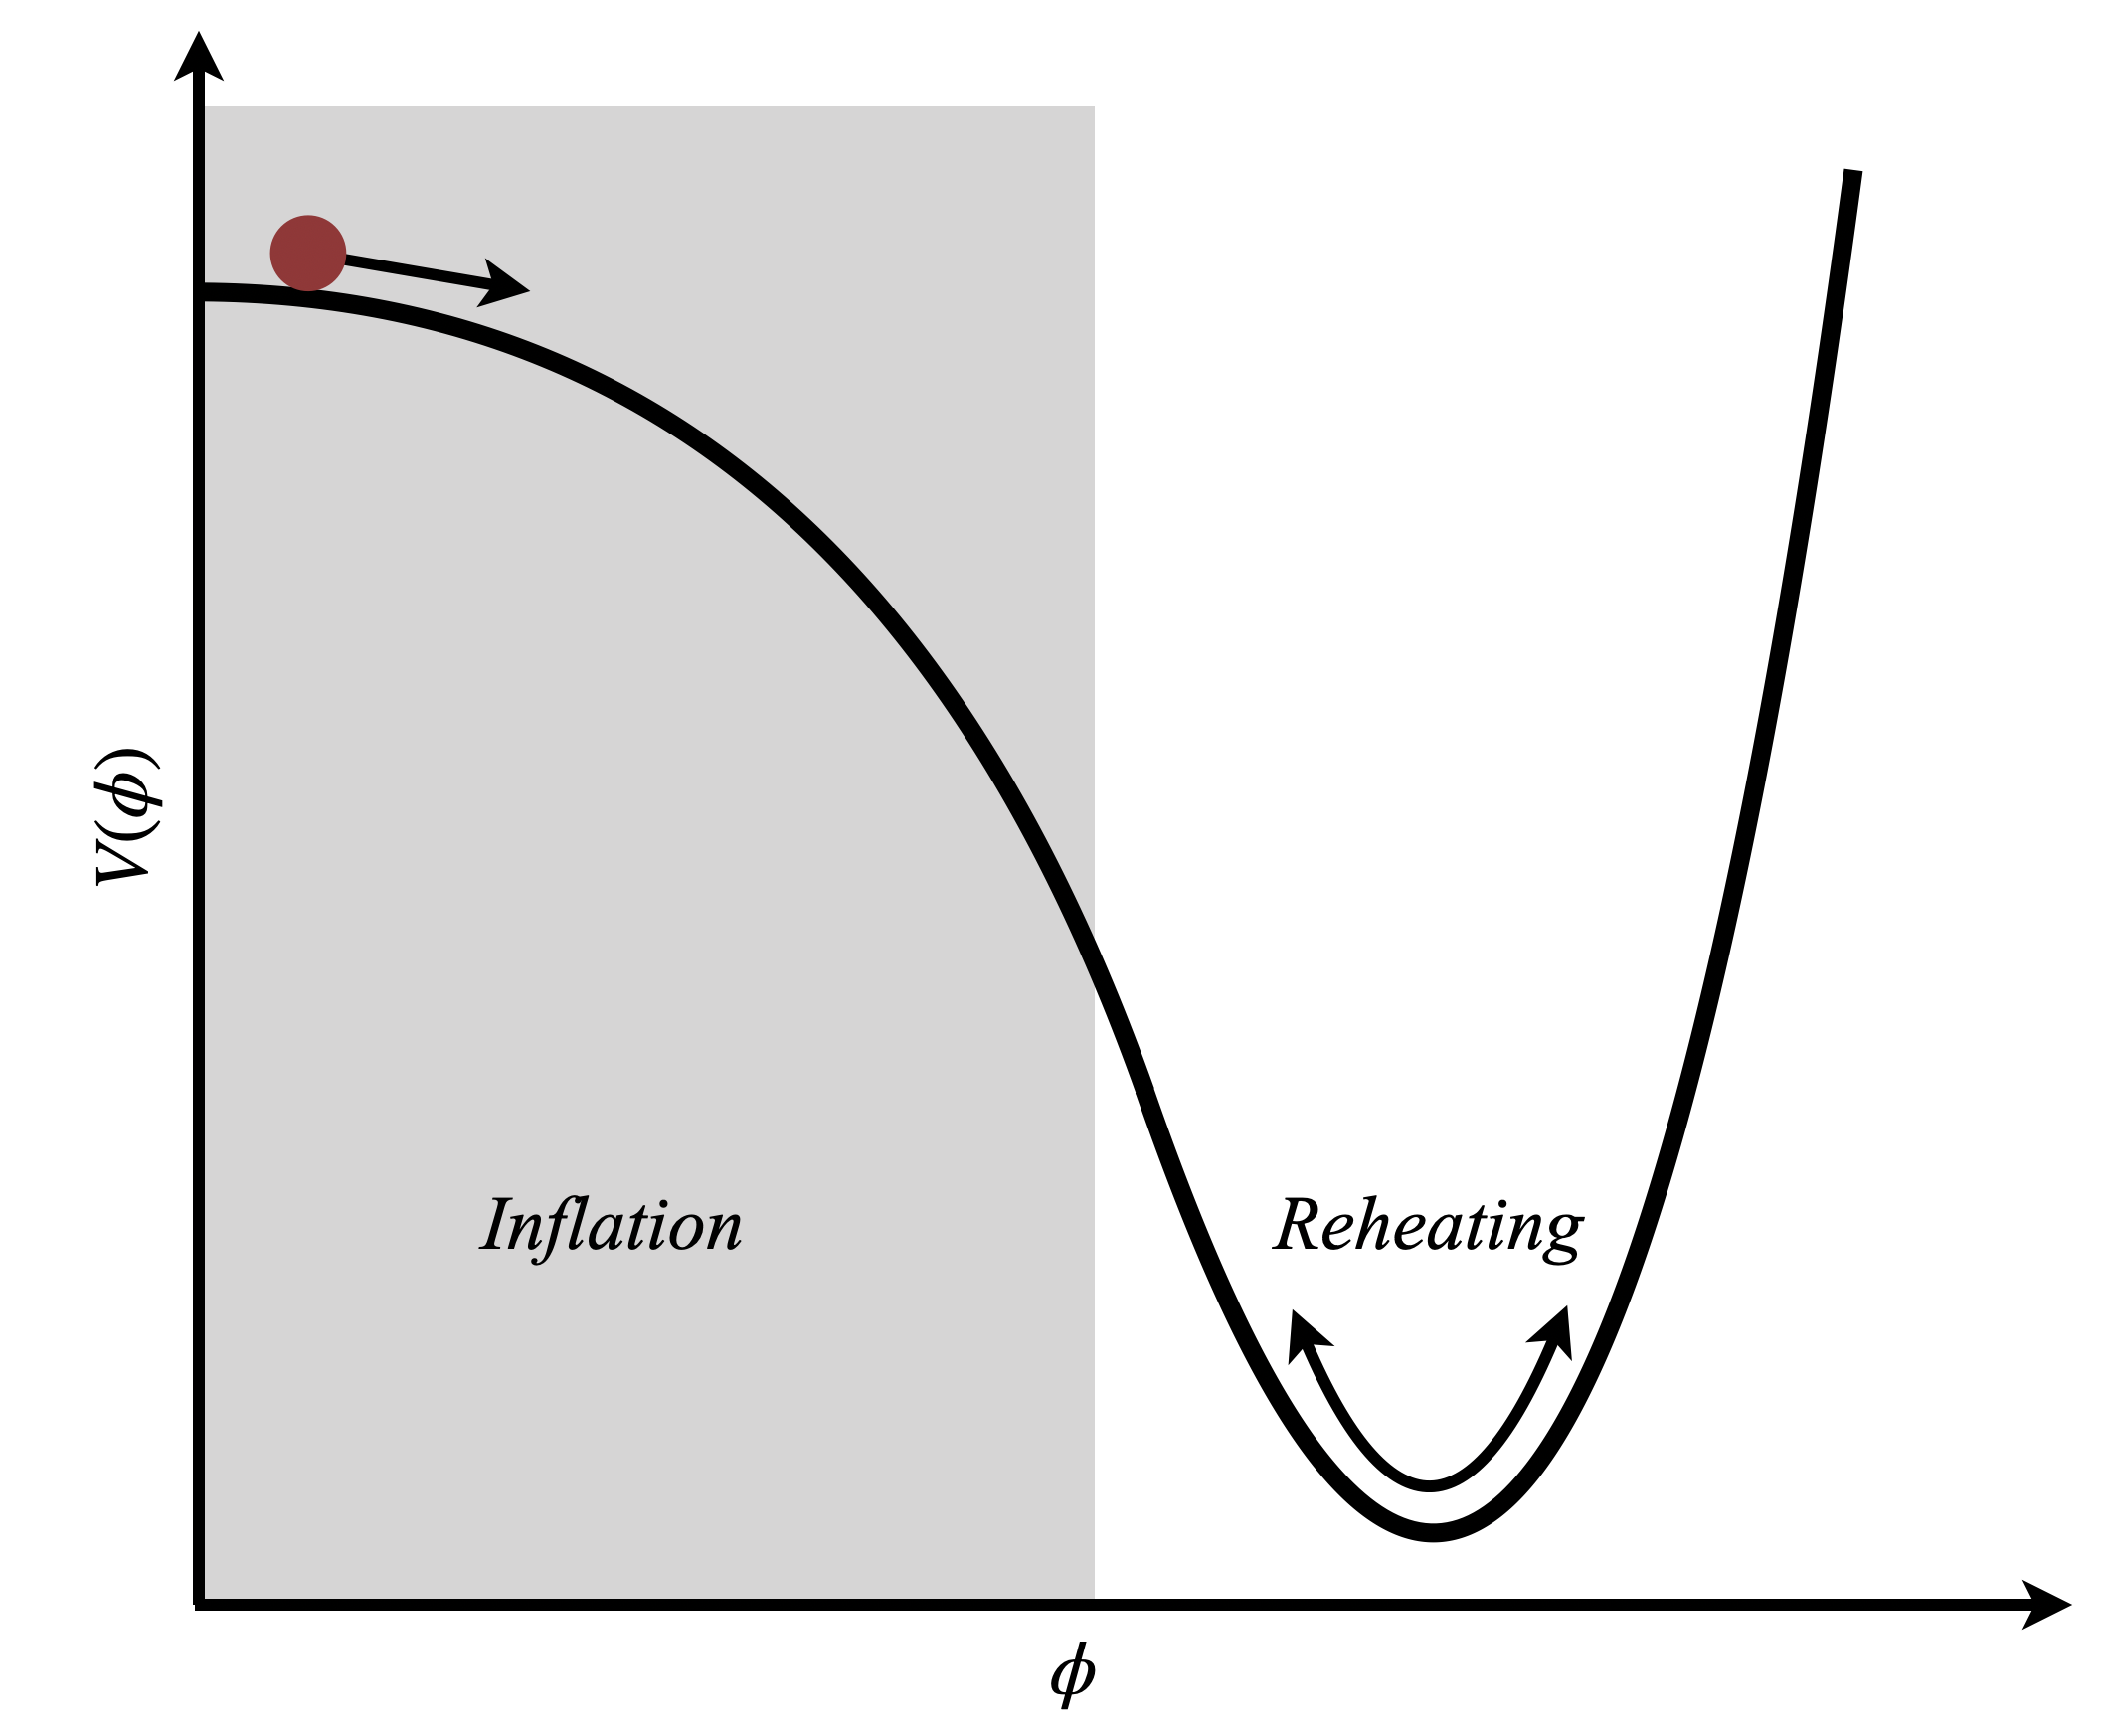
\includegraphics[height=6.6cm]{Figures/Chap_cosmo/SlowRoll2.png}\hfill
    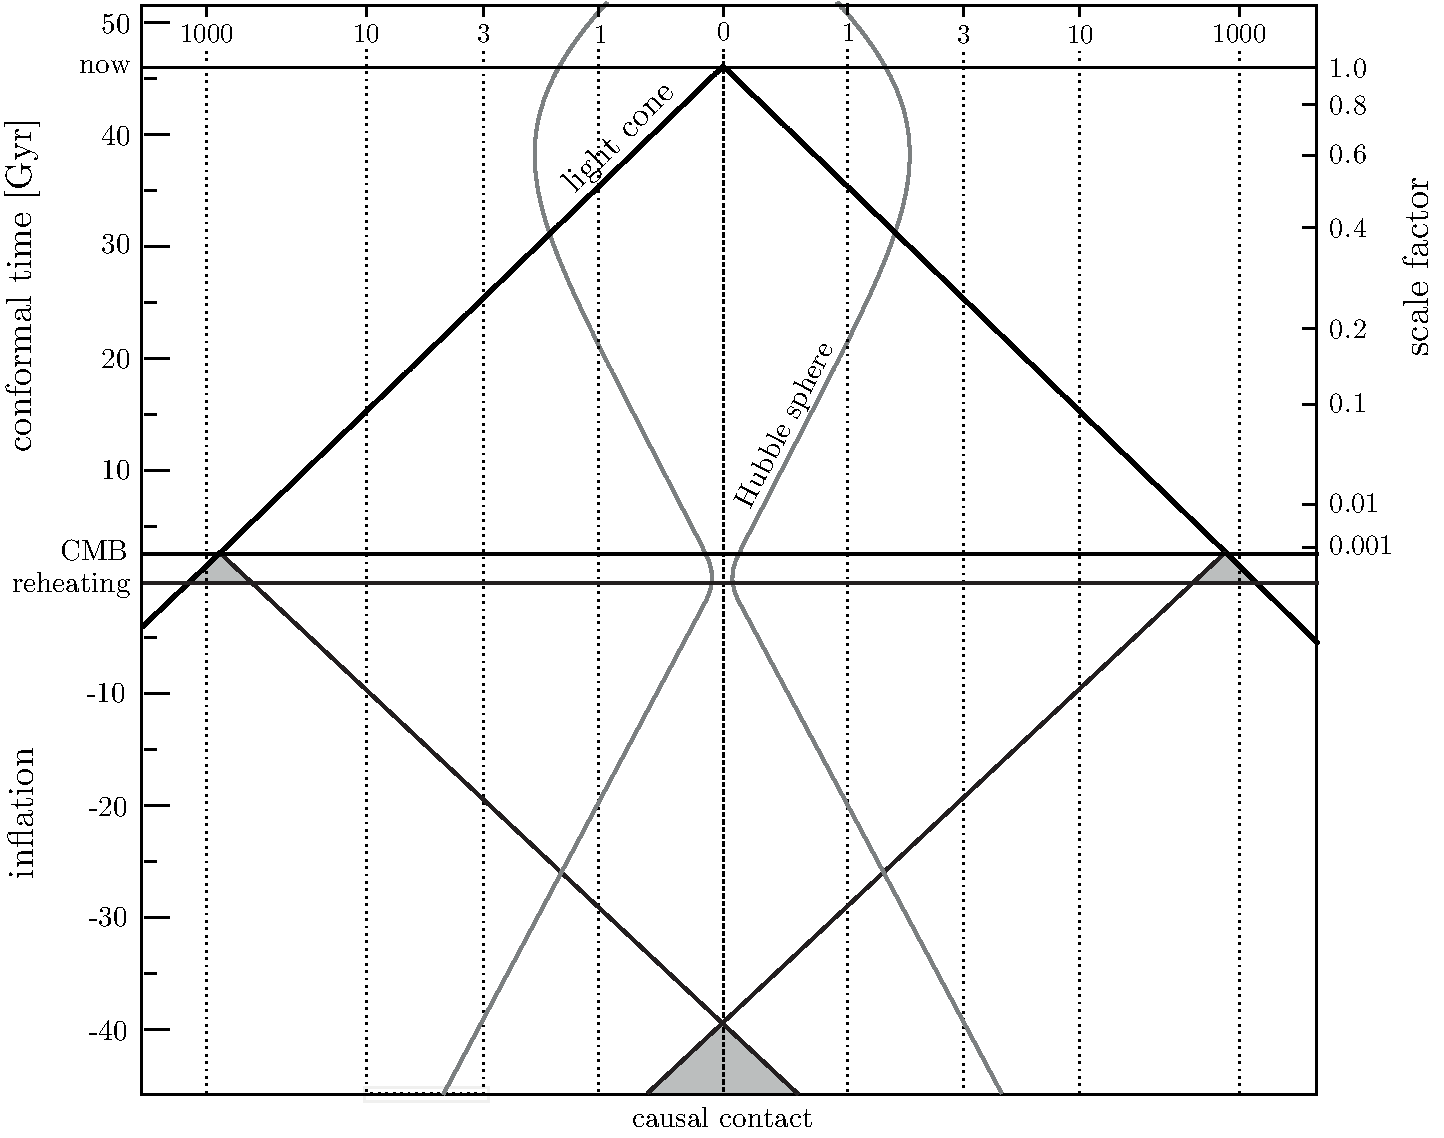
\includegraphics[height=6.6cm]{Figures/Chap_cosmo/spacetime_inflation.pdf}
    \caption{
        \textbf{Gauche:} Exemple de comportement du champ d'inflaton illustrant les deux régimes de l'équation (\ref{eq:infla_mvt}): le champ commence en \textit{slow roll} dans une région de potentiel élevé, puis se stabilise dans une région de bas potentiel, avec des oscillations rapides correspondant au \textit{reheating}.
        \textbf{Droite:} Diagramme d'espace-temps illustrant le contact causal de régions opposées dans le CMB au début de l'inflation.
        Figure extraite de \cite{baumann_inflation_2015}.
    }
    \label{fig:inflation}
\end{figure*}

La dynamique de l'inflation permet de comprendre la raison pour laquelle elle résout les problèmes de la platitude, de l'horizon et de l'hétérogénéité.
La densité d'énergie correspondant à la courbure de l'Univers étant définie par $\Omega_k = -kc^2 / (aH)^2$, celle-ci diminue rapidement avec le facteur d'échelle.
Quantitativement, en introduisant le nombre de \textit{e-folds} $N_e$, quantifiant l'augmentation du facteur d'échelle au cours de la phase inflationnaire, comme
\begin{equation}
    N_e = \ln \frac{a_f}{a_i} = \int_{t_i}^{t_f} H(t) \d t,
\end{equation}
il aparaît que $N_e \sim 60$ permet de passer d'une courbure $\Omega_k \sim 1$ au début de l'inflation à $\Omega_k \sim 10^{-60}$ à son issue, condition requise pour observer une courbure actuelle aussi faible que celle mesurée par le satellite \textit{Planck}.
De plus, le rayon de Hubble diminue pendant la phase inflationnaire, permettant à des points diamétralement opposés dans le CMB d'avoir été en contact causal.
Cela permet donc d'expliquer l'homogénéité du CMB, comme illustré sur le panneau droit de la figure \ref{fig:inflation}.

Enfin, le champ d'inflaton permet de comprendre l'origine des fluctuations de densité dans l'Univers primordial: considérons des fluctuations quantiques du champ comme une perturbation au premier ordre, soit
\begin{equation}
    \varphi(\xt) = \bar{\varphi}(t) + \delta\varphi(\xt),
\end{equation}
où $\bar{\varphi}(t)$ est la valeur moyenne du champ dans l'espace, ne dépendant que du temps dans l'hypothèse d'homogénéité. \\
Il apparait alors que la valeur du champ et de son potentiel ne sont pas égales en tout point de l'espace.
En vertu du lien entre densité d'énergie et espace-temps décrit par les équations d'Einstein (\ref{eq:einst_field}), ces inhomogénéités créent des perturbations dans la métrique de l'Univers, qui génèrent à leur tour des fluctuations dans la densité d'énergie du plasma primordial.
Ainsi, en plus des problèmes de l'horizon et de la platitude, l'inflation offre une origine au processus de formation des structures, qui sera détaillée dans la section suivante.

% ===================================================================================== %
\section{Évolution des grandes structures}

% ------------------------------------------------------------------------------------- %
\subsection{Croissance des inhomogénéités de densité}

Nous avons vu dans la section précédente comment l'inflation permettait de générer des fluctuations de densité dans l'Univers primordial.
Celles-ci seront ensuite amplifiées au cours de l'évolution de l'Univers par effondrement gravitationnel de la matière vers les régions les plus denses.
Ce processus de formation des structures est à l'origine des galaxies et de la distribution à grande échelle de la matière dans l'Univers contemporain, formant la toile cosmique.
Cette section détaille ce formalisme dans le but de comprendre l'origine des amas de galaxies, qui constituent la sonde cosmologique étudiée dans cette thèse.

Dans le régime linéaire, les fluctuations de densité issues de l'inflation peuvent s'écrire comme une perturbation au premier ordre de la densité moyenne,
\begin{equation}
    \label{eq:contrast}
    \rho(\xt) = \bar{\rho}(t) \left[1 + \delta(\xt) \right],
\end{equation}
où $\bar{\rho}(t)$ est la densité moyenne de l'Univers, $\vec{x}$ les coordonnées comobiles\footnotemark\ tri-dimensionelles, et $\delta(\xt)$ est appelé le paramètre de contraste. \\
\footnotetext{Le système de coordonnées comobiles se dilate avec le temps suivant l'expansion de l'Univers.}
La densité moyenne de l'Univers ne dépend que du temps, traduisant l'hypothèse d'un univers homogène à grande échelle et hétérogène seulement aux petites échelles.
Le fluide parfait comobile composant l'Univers doit alors satisfaire aux équations d'Euler, de la continuité, et de Poisson:
\begin{equation}
    \pdv{\vec{v}}{t} + (\vec{v} \cdot \vec{\nabla}) \vec{v} = -\vec{\nabla}\varphi - \frac{\vec{\nabla}p}{\rho} \label{eq:cosmo:euler}
\end{equation}
\begin{equation}
    \pdv{\rho}{t} + \vec{\nabla} \cdot (\rho \vec{v}) = 0 \label{eq:cosmo:conti}
\end{equation}
\begin{equation}
    \nabla^2 \Phi = 4\pi G \rho \label{eq:cosmo:poisson}
\end{equation}
où $p$ est la pression des fluides, $\vec{v}$ leur vitesse, et $\Phi$ le potentiel gravitationnel. \\
En injectant l'expression de la densité perturbée (\ref{eq:contrast}) dans ces équations, et en les combinant, on trouve l'expression de l'évolution des perturbations dans le temps:
\begin{equation}
    \pdvsq{\delta(\xt)}{t} + 2H(t)\pdv{\delta(\xt)}{t} = \left[4\pi G \bar{\rho}(t) + \frac{c_s^2}{a^2} \nabla^2\right] \delta(\xt),
\end{equation}
où $c_s$ est la vitesse du son dans le fluide. \\
Dans l'espace de Fourier, et en définissant $\delta_k {\rm sin}(\vec{k}\cdot\vec{r}) = \delta(\xt)$, cette équation prend la forme
\begin{equation}
    \ddot{\delta}_k + 2H\dot{\delta}_k = \left[4\pi G \bar{\rho} - \frac{c_s^2}{a^2} k^2\right] \delta_k
\end{equation}
ou encore, en introduisant l'échelle de Jeans $\lambda_{\rm J} \equiv c_s / \sqrt{\pi / G\bar{\rho}}$ et le mode associé $k_{\rm J} =2\pi a/\lambda_{\rm J}$,
\begin{equation}
    \label{eq:cosmo:delta_k}
    \ddot{\delta}_k + 2H\dot{\delta}_k = \frac{c_s^2}{a^2} (k_{\rm J}^2 - k^2) \delta_k.
\end{equation}

Deux régimes asymptotiques apparaissent.
Pour les perturbations plus grandes que l'échelle de Jeans, soit $k^2 \ll k_{\rm J}^2$, la gravitation domine l'évolution des perturbations, et leur croissance est permise.
À l'inverse, lorsque $k^2 \gg k_{\rm J}^2$, la pression domine l'effondrement gravitationnel et la croissance des perturbations est atténuée.
Ainsi, lorsque la densité d'énergie est partagée entre matière et rayonnement (dans l'Univers primordial, à $z \lesssim 3000$), les inhomogénéités de densité oscillent, augmentant sous domination de la force gravitationnelle, puis diminuant lorsque cette dernière devient faible devant les forces de pression.
Ce mécanisme empêche le développement des inhomogénéités au cours de l'ère du rayonnement.

Lorsque la matière domine la densité d'énergie de l'Univers, soit $a(t) \propto t^{2/3}$ d'après l'équation de Friedmann (\ref{eq:fried1}), les forces de pression deviennent négligeables, autorisant la croissance des inhomogénéités et la formation des structures.
La résolution de l'équation (\ref{eq:cosmo:delta_k}) montre alors que le contraste augmente comme $\delta(t) \propto t^{2/3}$.
Plus tard, lors de la domination de l'énergie sombre, le facteur d'échelle croît comme $a(t) \propto {\rm exp}(Ht)$, et la résolution de (\ref{eq:cosmo:delta_k}) montre une diminution du paramètre de contraste comme $\delta(t) \propto {\rm exp}(-2Ht)$.

% ------------------------------------------------------------------------------------- %
\subsection{Spectre de puissance de la distribution de matière}

Comme nous l'avons vu dans la section précédente, la distribution de densité de l'Univers primordial résulte d'un processus aléatoire, et la structure de l'Univers contemporain du développement de ces inhomogénéités.
Dans le cas de fluctuations gaussiennes, la distribution de densité primordiale peut se résumer à la fonction de corrélation du paramètre de contraste,
\begin{equation}
    \xi(\vec{r}) = \left< \delta(\vec{x} + \vec{r}) \delta(\vec{r}) \right>,
\end{equation}
où $\left< \cdots \right>$ représente la valeur moyenne prise en toute position $\vec{x}$ de l'Univers. \\
On peut encore définir le spectre de puissance primordial $P_{\rm prim.}(k)$ comme la transformée de Fourier de cette fonction de corrélation,
\begin{equation}
    P_{\rm prim.}(k) = \int \xi(\vec{r}) e^{-i \vec{k} \cdot \vec{r}} \, \d^3 \vec{r}.
\end{equation}
Les contraintes observationnelles sur le spectre de puissance primordial, obtenues notamment à partir de l'analyse des anisotropies du CMB, favorisent une forme en loi de puissance de ce dernier, soit $P(k) \propto k^n$, avec $n \simeq 1$ \cite{planck_collaboration_planck_2020}.
Le cas où $n = 1$ donne le spectre dit de Harrison-Zeldovich \cite{harrison_fluctuations_1970,zeldovich_hypothesis_1972}, qualifié d'invariant d'échelle.
En effet, en vertu de l'équation de Poisson, un spectre de puissance de la densité de matière de la forme $P(k) \propto k$ mène à un spectre de puissance du potentiel gravitationnel plat.

Dans l'Univers contemporain, les inhomogénéités de densité proviennent de l'accroissement des fluctuations primordiales.
Le spectre de puissance de la distribution de matière observable à un redshift $z$ est donc étroitement lié au spectre de puissance primordial, à travers
\begin{equation}
    P(z, k) = P_{\rm prim.}(k) \times T^2(z, k),
\end{equation}
où $T(z, k)$ est la fonction de transfert caractérisant l'évolution des perturbations. \\
La variance de la distribution de matière dans une sphère de rayon $r$ à un redshift $z$ est alors donnée par:
\begin{equation}
    \label{eq:matter_fluct}
    \sigma^2(z, r) = \frac{1}{(2\pi)^3} \int W(kr) P(z, k) \, \d^3k,
\end{equation}
où $W(kr)$ est la fonction fenêtre utilisée pour lisser la distribution de matière; par exemple, la fonction \textit{top-hat} considérant une sphère de rayon $r$,
\begin{equation}
    \label{eq:tophat}
    W(kr) = 3 \frac{\sin kr}{(kr)^3} - 3 \frac{\cos kr}{(kr)^2}.
\end{equation}
L'équation (\ref{eq:matter_fluct}) permet de définir le paramètre cosmologique $\sigma_8$ comme l'amplitude moyenne des fluctuations dans une sphère de $8 \, h^{-1}\, {\rm Mpc}$, soit
\begin{equation}
    \label{eq:sigma8}
    \sigma_8 = \sqrt{\sigma^2(z=0, r=8 \, h^{-1}\, {\rm Mpc})}.
\end{equation}
Ce paramètre a été mesuré par l'analyses des anisotropies primaires du CMB vues par \textit{Planck} à une valeur de $\sigma_8 = 0.8102 \pm  0.006$ \cite{planck_collaboration_planck_2020}.
Nous discuterons des différentes mesures obtenues par d'autres sondes en \mypageref{sec:current_surveys}.

% ------------------------------------------------------------------------------------- %
\subsection{Fonction de masse et distribution de halos}\label{sec:cosmo_hmf}

Le formalisme développé jusqu'ici repose sur l'hypothèse de linéarité des inhomogénéités du champ de matière primordial: d'après l'équation (\ref{eq:contrast}), les surdensités représentent des perturbations au premier ordre d'un Univers globalement homogène.
Cette hypothèse suppose donc que $\delta \ll 1$, condition non-remplie dans les surdensités de l'Univers contemporain.
Par exemple, les amas de galaxies peuvent aujourd'hui atteindre des densités centrales de l'ordre de $\sim 10^{-22} \;{\rm kg \cdot m^{-3}}$, correspondant à un contraste de l'ordre de $10^4$.
La description de l'Univers contemporain par le seul formalisme de la croissance des structures par développement des inhomogénéités en régime linéaire est donc incomplète.

Les phénomènes physiques devant être pris en compte lors du traitement non-linéaire de la croissance des structures sont très riches, et font de ce formalisme un cadre complexe.
Une approche possible est la théorie de \myciteauthor{press_formation_1974}, dans laquelle l'hypothèse principale est le fait que l'intégralité de la matière est aujourd'hui contenue dans des halos sphériques à l'équilibre hydrostatique.
Dans le cadre de cette théorie, le nombre de halos de masse comprise dans un intervalle $[M, M + \d M]$ est donné par la fonction de masse $\d N / \d M$.
Dans sa formulation courante, formalisée par \myciteauthor{tinker_toward_2008}, celle-ci s'écrit à un redshift donné:
\begin{equation}
    \label{eq:hmf}
    \frac{\d N}{\d M} = f(\sigma) \frac{\bar{\rho}}{M} \left| \frac{\d \, {\rm ln}\, \sigma^{-1}}{\d M} \right|,
\end{equation}
où $\bar{\rho}$ est la densité moyenne de l'Univers, $\sigma$ la racine de la variance de la distribution de matière, reliée au spectre de puissance par l'équation (\ref{eq:matter_fluct}), et $f(\sigma)$ est la fonction de multiplicité dépendant de $\sigma$, par
\begin{equation}
    f(\sigma) = A \left[ 1 + \left(\frac{b}{\sigma}\right)^a \right] e^{-c / \sigma^2}
\end{equation}
Les valeurs des paramètres $(A, a, b, c)$ de la fonction de multiplicité sont donc des paramètres de la fonction de masse, et sont généralement mesurés dans des simulations numériques (\eg\ \cite{tinker_toward_2008,bocquet_halo_2016,bocquet_mira-titan_2020}).
Comme nous le verrons dans le chapitre suivant, la fonction de masse est un élément central des analyses cosmologiques basées sur les amas de galaxies.
En effet, elle dépend de la distribution de matière dans l'Univers, et donc des paramètres cosmologiques.

C'est cette dépendance, illustrée en figure \ref{fig:hmf_cosmo}, qui est exploitée pour contraindre la cosmologie à l'aide d'amas de galaxies.
Celle-ci montre l'évolution des valeurs de la fonction de masse de \myciteauthor{tinker_toward_2008} avec les paramètres $\Omega_m$ et $\sigma_8$.
On y observe que la fonction de masse croît avec $\Omega_m$: plus la matière est abondante dans l'Univers (c'est-à-dire plus $\Omega_m$ est grand), plus les halos, et donc les amas de galaxies, sont nombreux\footnotemark.
On y remarque également un comportement similaire pour $\sigma_8$: plus les fluctuations de la distribution de matière sont grandes (c'est-à-dire plus $\sigma_8$ est grand), plus les amas sont nombreux.
On note enfin que les deux paramètres cosmologiques ont une influence différente sur l'abondance d'amas.
Une variation de $\Omega_m$ influera principalement sur l'abondance d'amas de faible masse, alors qu'à l'inverse, une variation de $\sigma_8$ modifiera surtout l'abondance d'amas massifs.
Les contraintes basées sur l'abondance d'amas sont de fait sensibles à une combinaison des deux paramètres, pouvant varier d'une analyse à l'autre, et souvent exprimée par le paramètre $S_8$:
\begin{equation}
    S_8 \equiv \sigma_8 \sqrt{\Omega_m/0.3}.
\end{equation}
\footnotetext{Cette observation n'est plus vraie pour les objets extrêmement massifs, au delà de $2 \times 10^{15} \, M_\odot$ à $z=0.5$. On note que de tels objets sont des cas extrêmes; leur existence seule pousserait le modèle $\Lambda{\rm CDM}$ à ses limites, et des objets plus massifs pourrait même permettre de l'invalider -- voir par exemple \cite{harrison_consistent_2013}.}

La connaissance de la fonction de masse est donc une nécessité pour la justesse des analyses cosmologiques basées sur les statistiques d'amas (\eg\ \cite{salvati_impact_2020,artis_impact_2021}).
De telles analyses seront détaillées au chapitre suivant, et en particulier en section \mypageref{sec:cluster_nbcount}.

\begin{figure*}[t]
    \centering
    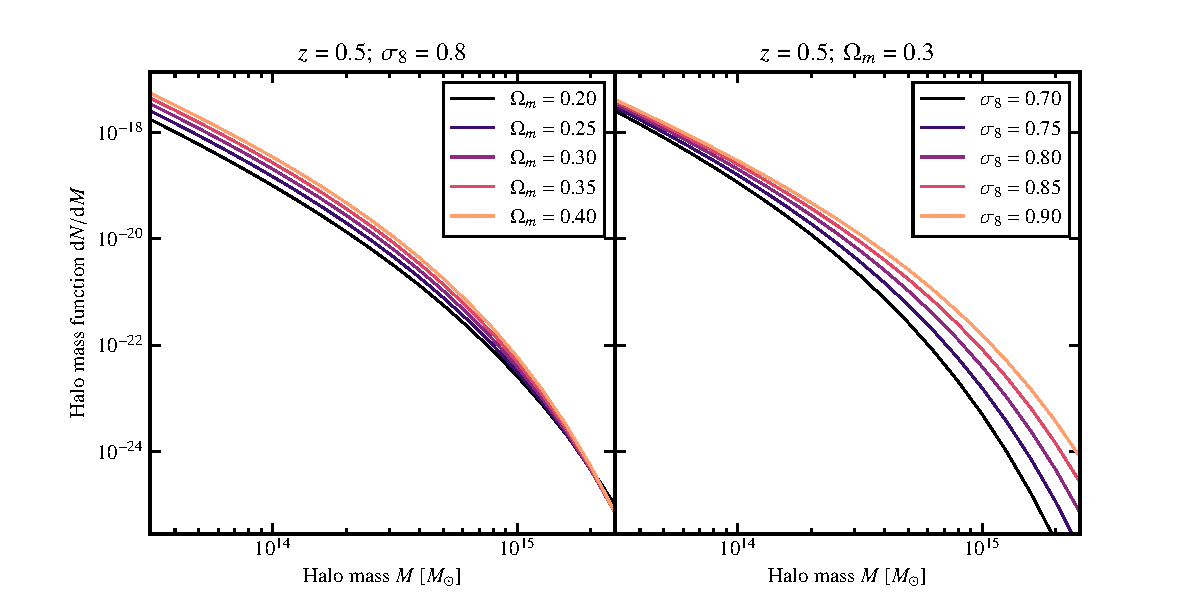
\includegraphics[width=\linewidth]{Figures/Chap_cosmo/hmf_cosmo.pdf}
    \caption{
        Illustration de l'évolution de la fonction de masse avec les paramètres cosmologiques.
        La fonction de masse de \myciteauthor{tinker_toward_2008} est représentée pour différentes valeurs de $\Omega_m$ (\textit{gauche}), et de $\sigma_8$ (\textit{droite}).
        Le redshift est fixé à $z = 0.5$.
    }
    \label{fig:hmf_cosmo}
\end{figure*}

% ===================================================================================== %
\section{Conclusions}

Le modèle standard de la cosmologie, accompagné du paradigme de l'inflation, fournit une description de l'Univers et de son évolution basée sur des hypothèses simples.
À l'heure actuelle, il est en remarquable accord avec les observations disponibles.
Cependant, plusieurs questions restent en suspens.
Par exemple, la nature de l'énergie sombre, cause de l'accélération récente de l'expansion, est une des énigmes non-résolues par le modèle $\Lambda {\rm CDM}$.
La mesure de son paramètre d'équation d'état, et de son éventuelle évolution dans le temps, peut apporter des réponses à cette question.

La mesure toujours plus précise des valeurs des paramètres cosmologiques est l'un des enjeux majeurs de la cosmologie moderne.
Dans ce but, la combinaison de plusieurs observables, nommées \textit{sondes cosmologiques}, s'impose comme un puissant moyen de mitiger les différentes incertitudes systématiques associées à chacune des sondes individuelles.
Plusieurs études récentes semblent indiquer un désaccord entre les mesures des paramètres cosmologiques effectuées avec différentes sondes.
Par exemple, les mesures du taux actuel d'expansion de l'Univers $H_0$ réalisées par l'analyse des anisotropies du CMB sont en désaccord avec les mesures réalisées dans l'Univers contemporain (voir par exemple \cite{riess_large_2019,wong_h0licow_2020,efstathiou_h0_2021, freedman_measurements_2021}).
On note également la différence entre les estimations du paramètre $S_8$ par l'analyse du CMB et d'autres sondes, qui sera discutée au chapitre suivant.
Ces tensions peuvent être un signe de nouvelle physique, ou bien indiquer des effets systématiques non-maîtrisés.
Alors même que les incertitudes statistiques s'apprêtent à être réduites de manière conséquente avec les différents relevés cosmologiques du futur, ces systématiques deviendront de plus en plus importantes, et devront être étudiées afin de pouvoir répondre aux questions toujours ouvertes sur les propriétés les plus fondamentales de l'Univers.
Cette thèse s'inscrit dans le cadre de l'étude de ces effets systématiques dans l'exploitation cosmologique des amas de galaxies, qui sera décrite dans le chapitre suivant.
